\documentclass[]{article}
\usepackage{lmodern}
\usepackage{amssymb,amsmath}
\usepackage{ifxetex,ifluatex}
\usepackage{fixltx2e} % provides \textsubscript
\ifnum 0\ifxetex 1\fi\ifluatex 1\fi=0 % if pdftex
  \usepackage[T1]{fontenc}
  \usepackage[utf8]{inputenc}
\else % if luatex or xelatex
  \ifxetex
    \usepackage{mathspec}
  \else
    \usepackage{fontspec}
  \fi
  \defaultfontfeatures{Ligatures=TeX,Scale=MatchLowercase}
\fi
% use upquote if available, for straight quotes in verbatim environments
\IfFileExists{upquote.sty}{\usepackage{upquote}}{}
% use microtype if available
\IfFileExists{microtype.sty}{%
\usepackage{microtype}
\UseMicrotypeSet[protrusion]{basicmath} % disable protrusion for tt fonts
}{}
\usepackage[margin=1in]{geometry}
\usepackage{hyperref}
\hypersetup{unicode=true,
            pdftitle={Supplementary Material},
            pdfauthor={Lucas Henriques Viscardi; Danilo Oliveira Imparato; Maria Cátira Bortolini; Rodrigo Juliani Siqueira Dalmolin},
            pdfkeywords={Evolution; Nervous system},
            pdfborder={0 0 0},
            breaklinks=true}
\urlstyle{same}  % don't use monospace font for urls
\usepackage{graphicx,grffile}
\makeatletter
\def\maxwidth{\ifdim\Gin@nat@width>\linewidth\linewidth\else\Gin@nat@width\fi}
\def\maxheight{\ifdim\Gin@nat@height>\textheight\textheight\else\Gin@nat@height\fi}
\makeatother
% Scale images if necessary, so that they will not overflow the page
% margins by default, and it is still possible to overwrite the defaults
% using explicit options in \includegraphics[width, height, ...]{}
\setkeys{Gin}{width=\maxwidth,height=\maxheight,keepaspectratio}
\IfFileExists{parskip.sty}{%
\usepackage{parskip}
}{% else
\setlength{\parindent}{0pt}
\setlength{\parskip}{6pt plus 2pt minus 1pt}
}
\setlength{\emergencystretch}{3em}  % prevent overfull lines
\providecommand{\tightlist}{%
  \setlength{\itemsep}{0pt}\setlength{\parskip}{0pt}}
\setcounter{secnumdepth}{0}
% Redefines (sub)paragraphs to behave more like sections
\ifx\paragraph\undefined\else
\let\oldparagraph\paragraph
\renewcommand{\paragraph}[1]{\oldparagraph{#1}\mbox{}}
\fi
\ifx\subparagraph\undefined\else
\let\oldsubparagraph\subparagraph
\renewcommand{\subparagraph}[1]{\oldsubparagraph{#1}\mbox{}}
\fi

%%% Use protect on footnotes to avoid problems with footnotes in titles
\let\rmarkdownfootnote\footnote%
\def\footnote{\protect\rmarkdownfootnote}

%%% Change title format to be more compact
\usepackage{titling}

% Create subtitle command for use in maketitle
\providecommand{\subtitle}[1]{
  \posttitle{
    \begin{center}\large#1\end{center}
    }
}

\setlength{\droptitle}{-2em}

  \title{Supplementary Material}
    \pretitle{\vspace{\droptitle}\centering\huge}
  \posttitle{\par}
  \subtitle{Ionotropic receptors as the driving force behind human synapse
establishment}
  \author{Lucas Henriques Viscardi \\ Danilo Oliveira Imparato \\ Maria Cátira Bortolini \\ Rodrigo Juliani Siqueira Dalmolin}
    \preauthor{\centering\large\emph}
  \postauthor{\par}
    \date{}
    \predate{}\postdate{}
  
\usepackage{docmute}

\begin{document}
\maketitle
\begin{abstract}
Model uncertainty and limited data are fundamental challenges to robust
management of human intervention in a natural system. These challenges
are acutely highlighted by concerns that many ecological systems may
contain tipping points, such as Allee population sizes. Before a
collapse, we do not know where the tipping points lie, if they exist at
all. Hence, we know neither a complete model of the system dynamics nor
do we have access to data in some large region of state-space where such
a tipping point might exist.
\end{abstract}

{
\setcounter{tocdepth}{6}
\tableofcontents
}
\hypertarget{project-structure}{%
\section{Project structure}\label{project-structure}}

This is the title page

\hypertarget{preprocessing}{%
\section{Preprocessing}\label{preprocessing}}

Preprocessing

\hypertarget{eukaryota-species-tree}{%
\subsection{Eukaryota species tree}\label{eukaryota-species-tree}}

Explanation

\hypertarget{ncbi-taxonomy-tree}{%
\subsubsection{NCBI Taxonomy tree}\label{ncbi-taxonomy-tree}}

Explanation

\hypertarget{duplicated-genera}{%
\subsubsection{Duplicated Genera}\label{duplicated-genera}}

\hypertarget{hybrid-tree}{%
\subsubsection{Hybrid tree}\label{hybrid-tree}}

Explanation

\hypertarget{gene-selection-and-annotation}{%
\subsection{Gene selection and
annotation}\label{gene-selection-and-annotation}}

\hypertarget{gene-selection-and-annotation-1}{%
\subsection{Gene selection and
annotation}\label{gene-selection-and-annotation-1}}

\hypertarget{neuroexclusivity}{%
\subsection{Neuroexclusivity}\label{neuroexclusivity}}

Explanation

\hypertarget{expression}{%
\subsubsection{Expression}\label{expression}}

\hypertarget{pathways}{%
\subsubsection{Pathways}\label{pathways}}

\hypertarget{cog-data}{%
\subsection{COG data}\label{cog-data}}

\hypertarget{network}{%
\subsection{Network}\label{network}}

\hypertarget{analysis}{%
\section{Analysis}\label{analysis}}

Analysis

\begin{Shaded}
\begin{Highlighting}[]
\KeywordTok{library}\NormalTok{(here)}
\end{Highlighting}
\end{Shaded}

\begin{verbatim}
## here() starts at /home/danilo/R/neuro
\end{verbatim}

\begin{Shaded}
\begin{Highlighting}[]
\KeywordTok{library}\NormalTok{(purrr)}
\KeywordTok{library}\NormalTok{(tibble)}

\KeywordTok{library}\NormalTok{(knitr)}
\KeywordTok{library}\NormalTok{(kableExtra)}

\CommentTok{# download_if_missing <- function(filename, url) \{}
\CommentTok{#   if (!file.exists(here("data-raw", "download", filename))) \{}
\CommentTok{#     download.file(url, filename)}
\CommentTok{#   \}}
\CommentTok{# \}}

\CommentTok{# files <- tribble(}
\CommentTok{#   ~filename,           ~url,}
\CommentTok{#   "species.v11.0.txt", "https://stringdb-static.org/download/species.v11.0.txt",}
\CommentTok{#   # "download/taxonomy", "https://ftp.ncbi.nlm.nih.gov/pub/taxonomy/new_taxdump/new_taxdump.tar.gz",}
\CommentTok{#   # "x",                 "y",}
\CommentTok{#   # "x",                 "y",}
\CommentTok{# )}

\NormalTok{files <-}\StringTok{ }\KeywordTok{tribble}\NormalTok{(}
  \OperatorTok{~}\NormalTok{url,}
  \OperatorTok{~}\NormalTok{filename,}
  
  \StringTok{"https://stringdb-static.org/download/species.v11.0.txt"}\NormalTok{,}
  \StringTok{"species.v11.0.txt"}\NormalTok{,}
  
  \StringTok{"https://ftp.ncbi.nlm.nih.gov/pub/taxonomy/new_taxdump/new_taxdump.tar.gz"}\NormalTok{,}
  \StringTok{"new_taxdump.tar.gz"}\NormalTok{,}
  
  \StringTok{"http://rest.kegg.jp/link/pathway/hsa"}\NormalTok{,}
  \StringTok{"link_pathway_entrez.tsv"}\NormalTok{,}
  
  \StringTok{"https://string-db.org/mapping_files/entrez/human.entrez_2_string.2018.tsv.gz"}\NormalTok{,}
  \StringTok{"human.entrez_2_string.2018.tsv.gz"}\NormalTok{,}
  
  \StringTok{"https://string-db.org/mapping_files/STRING_display_names/human.name_2_string.tsv.gz"}\NormalTok{,}
  \StringTok{"human.name_2_string.tsv.gz"}\NormalTok{,}
  
  \StringTok{"https://ftp.ncbi.nlm.nih.gov/gene/DATA/GENE_INFO/Mammalia/Homo_sapiens.gene_info.gz"}\NormalTok{,}
  \StringTok{"Homo_sapiens.gene_info.gz"}\NormalTok{,}
  
  \StringTok{"http://rest.genome.jp/link/ensembl/hsa"}\NormalTok{,}
  \StringTok{"link_ensembl_entrez.tsv"}\NormalTok{,}
  
  \CommentTok{# "https://ftp.ncbi.nlm.nih.gov/gene/DATA/GENE_INFO/Mammalia/Homo_sapiens.gene_info.gz",}
  \CommentTok{# "Homo_sapiens.gene_info.gz",}
\NormalTok{)}

\NormalTok{files }\OperatorTok
\StringTok{  }\KeywordTok{kable}\NormalTok{(}\DataTypeTok{format =} \StringTok{"html"}\NormalTok{) }\OperatorTok
\StringTok{  }\KeywordTok{kable_styling}\NormalTok{(}\DataTypeTok{bootstrap_options =} \StringTok{"striped"}\NormalTok{)}
\end{Highlighting}
\end{Shaded}

url

filename

\url{https://stringdb-static.org/download/species.v11.0.txt}

species.v11.0.txt

\url{https://ftp.ncbi.nlm.nih.gov/pub/taxonomy/new_taxdump/new_taxdump.tar.gz}

new\_taxdump.tar.gz

\url{http://rest.kegg.jp/link/pathway/hsa}

link\_pathway\_entrez.tsv

\url{https://string-db.org/mapping_files/entrez/human.entrez_2_string.2018.tsv.gz}

human.entrez\_2\_string.2018.tsv.gz

\url{https://string-db.org/mapping_files/STRING_display_names/human.name_2_string.tsv.gz}

human.name\_2\_string.tsv.gz

\url{https://ftp.ncbi.nlm.nih.gov/gene/DATA/GENE_INFO/Mammalia/Homo_sapiens.gene_info.gz}

Homo\_sapiens.gene\_info.gz

\url{http://rest.genome.jp/link/ensembl/hsa}

link\_ensembl\_entrez.tsv

\begin{Shaded}
\begin{Highlighting}[]
\CommentTok{# pwalk(files, download_if_missing)}
\KeywordTok{plot}\NormalTok{(}\DecValTok{1}\NormalTok{,}\DecValTok{1}\NormalTok{)}
\end{Highlighting}
\end{Shaded}

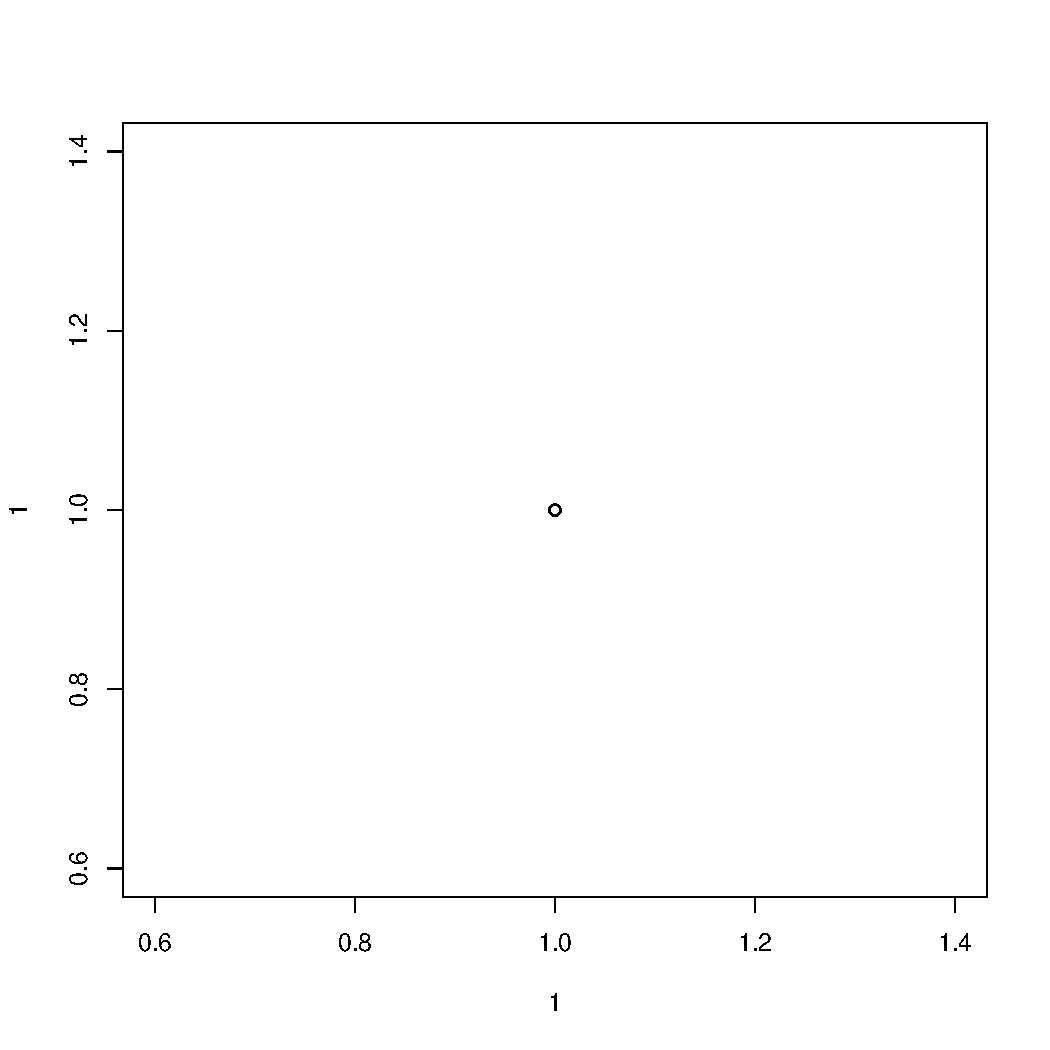
\includegraphics{figs/unnamed-chunk-2-1.pdf}

\hypertarget{special-cases}{%
\section{Special cases}\label{special-cases}}

\begin{Shaded}
\begin{Highlighting}[]
\CommentTok{# if (!file.exists("download/taxonomy")) \{}
\CommentTok{#   tmp <- tempfile()}
\CommentTok{#   download.file("https://ftp.ncbi.nlm.nih.gov/pub/taxonomy/new_taxdump/new_taxdump.tar.gz", tmp)}
\CommentTok{#   untar(tmp, exdir = "download/taxonomy")}
\CommentTok{#   unlink(tmp)}
\CommentTok{# \}}
\end{Highlighting}
\end{Shaded}




\end{document}
